% Toutes les valeurs viennent des sorties réelles du rejeu final sur Hive (resultats/sorties/).
% Une ligne "
% =====================================================================
\newpage
\section*{Introduction}
\phantomsection
\addcontentsline{toc}{section}{Introduction}

\noindent \textbf{Apache Hive} est un entrepôt de données bâti sur Hadoop. Il permet d'interroger des fichiers stockés dans HDFS avec le langage \textbf{HiveQL}, très proche du SQL~: Hive traduit chaque requête en travaux MapReduce. Hive sépare les données (des fichiers dans HDFS) de leur description (le \textit{metastore}, qui contient les noms de tables, les colonnes et les emplacements). Une table peut donc être de deux types~:
\begin{itemize}
	\item \textbf{externe} (\texttt{EXTERNAL})~: Hive ne décrit que des fichiers qui existent déjà. Supprimer la table ne supprime pas les fichiers~;
	\item \textbf{interne} (gérée)~: Hive possède les fichiers. Supprimer la table les supprime aussi.
\end{itemize}

\begin{center}
\begin{adjustbox}{max width=\linewidth}
\begin{tikzpicture}[node distance=1.7cm, every node/.style={font=\scriptsize}]
	\node[cmp=2.3cm] (cl) {\textbf{Client}\\ Hive CLI, Hue};
	\node[cmp=2.6cm, right=of cl] (dr) {\textbf{Driver HiveQL}\\ analyse, optimisation, plan};
	\node[cmp=2.6cm, right=of dr] (mr) {\textbf{Jobs MapReduce}\\ exécutés par YARN};
	\node[cmp=2.6cm, right=of mr, fill=title2!12, draw=title1] (hd) {\textbf{HDFS}\\ \texttt{/user/hive/...}};
	\node[cmp=2.6cm, below=1.2cm of dr, fill=gray!10, draw=gray] (ms) {\textbf{Metastore} (MySQL)\\ tables, colonnes, emplacements};
	\draw[flux] (cl) -- node[above]{requête} (dr);
	\draw[flux] (dr) -- node[above]{compile} (mr);
	\draw[flux] (mr) -- node[above]{lit, écrit} (hd);
	\draw[flux, dashed] (dr) -- node[right]{schéma} (ms);
	\draw[flux, dashed] (hd.south) |- node[pos=0.25, right]{fichiers} (ms.east);
\end{tikzpicture}
\end{adjustbox}\par\nobreak\smallskip
\small\textit{Figure~1 -- Architecture de Hive sur la machine Cloudera~: le metastore décrit les tables, HDFS contient les fichiers.}
\end{center}

\noindent Le compte-rendu commence par une étude des six fichiers de données, puis le workshop comporte trois parties~:
\begin{enumerate}
	\item créer une base et des tables, externes puis internes, et observer ce que devient le fichier à la suppression~;
	\item organiser les données avec des \textbf{partitions} et des \textbf{buckets}~;
	\item analyser les salaires d'une entreprise avec dix requêtes HiveQL.
\end{enumerate}

\noindent Tout est exécuté sur la machine virtuelle \textbf{Cloudera quickstart 5.12} (Hive 1.1.0-cdh5.12.0), avec un script par partie. Le script \texttt{00\_hdfs.sh} prépare les dossiers HDFS, puis \texttt{01\_base\_et\_tables.hql}, \texttt{02\_partitions\_buckets.hql} et \texttt{03\_analyse.hql} se lancent avec \texttt{hive -f}. Chaque fichier de données est placé dans son propre dossier HDFS~: une table externe lit tous les fichiers de son dossier.

% =====================================================================
\section*{Étude des données}
\phantomsection
\addcontentsline{toc}{section}{Étude des données}

\noindent Avant d'écrire une table, les six fichiers fournis ont été analysés~: leur forme décide du type des colonnes et des options de lecture. Le tableau donne leur contenu, puis les particularités à connaître.

\begin{tableau}{|>{\ttfamily\raggedright\arraybackslash}p{\dimexpr0.30\linewidth-2\tabcolsep-1.2\arrayrulewidth\relax}|>{\raggedleft\arraybackslash}p{\dimexpr0.08\linewidth-2\tabcolsep-1.2\arrayrulewidth\relax}|>{\raggedright\arraybackslash}p{\dimexpr0.40\linewidth-2\tabcolsep-1.2\arrayrulewidth\relax}|>{\raggedright\arraybackslash}p{\dimexpr0.22\linewidth-2\tabcolsep-1.2\arrayrulewidth\relax}|}
\rowcolor{tabentete}\normalfont \textbf{Fichier} & \normalfont \textbf{Lignes} & \normalfont \textbf{Contenu} & \normalfont \textbf{Utilisé en} \\ \hline
emploi\_population.txt & 12 & Genre, date de naissance, fonction, salaire, code postal, id & Partie 1 \\ \hline
personne.txt & 12 & Id, nom, prénoms & Partie 1 (table interne) \\ \hline
internautes\_log.txt & 17 & Id, prénom, site consulté, date, pays & Partie 2 \\ \hline
employes.txt & 33 & Id, nom, prénoms, date de naissance & Partie 3 \\ \hline
fonction\_employes.txt & 33 & Id, année d'embauche, fonction & Partie 3 \\ \hline
salaire\_employes.txt & 33 & Sexe, secteur, salaire, code postal, id & Partie 3 \\ \hline
\end{tableau}

\noindent Les nombres de lignes comptent les données, sans l'en-tête (\texttt{fonction\_employes.txt} et \texttt{salaire\_employes.txt} ont 34 lignes avec lui). Les volumes qui comptent pour la suite~:

\begin{itemize}
	\item \textbf{33 employés}, répartis en \textbf{16 secteurs} (partie~3)~;
	\item \textbf{17 lignes de journal}, sur \textbf{3 dates} (27, 28 et 29 avril 2016) et \textbf{6 pays} (partie~2)~;
	\item \textbf{12 personnes} dans les deux fichiers de la partie~1.
\end{itemize}

\noindent Les fichiers ont en commun leur séparateur, le point-virgule, écrit \texttt{'\textbackslash 073'} (son code octal) dans les scripts. Les autres caractéristiques diffèrent d'un fichier à l'autre~:

\begin{tableau}{|>{\bfseries\raggedright\arraybackslash}p{\dimexpr0.17\linewidth-2\tabcolsep-1.2\arrayrulewidth\relax}|>{\raggedright\arraybackslash}p{\dimexpr0.45\linewidth-2\tabcolsep-1.2\arrayrulewidth\relax}|>{\raggedright\arraybackslash}p{\dimexpr0.38\linewidth-2\tabcolsep-1.2\arrayrulewidth\relax}|}
\rowcolor{tabentete}\normalfont \textbf{Caractéristique} & \normalfont \textbf{Constat} & \normalfont \textbf{Conséquence pour Hive} \\ \hline
Encodage & \texttt{fonction\_employes.txt} et \texttt{salaire\_employes.txt} étaient en ISO-8859-1~; les quatre autres sont en ASCII & Accents illisibles (« profession juridique privé », « année-embauche ») tant qu'ils ne sont pas en UTF-8 \\ \hline
Fins de ligne & Les six fichiers d'origine étaient en CRLF & Hive garde le \texttt{\textbackslash r} dans la dernière colonne, ce qui donne \texttt{NULL} sur un entier \\ \hline
En-têtes & Une ligne d'en-tête dans \texttt{fonction\_employes.txt} et \texttt{salaire\_employes.txt} seulement & Cette ligne serait lue comme une donnée \\ \hline
Dates & \texttt{emploi\_population.txt}~: AAAA-MM-JJ~; \texttt{employes.txt}~: JJ/MM/AAAA~; \texttt{internautes\_log.txt}~: JJ-MM-AAAA & Seul le premier format est accepté par le type \texttt{DATE} \\ \hline
Salaire & Une chaîne du type \texttt{20000euro/an}, avec une faute à la ligne~26 (\texttt{42000euo/an}) & Pas de calcul possible sans extraire les chiffres \\ \hline
\end{tableau}

\noindent Le traitement appliqué à chacun de ces points est détaillé dans la section « Pièges des données et écarts à l'énoncé ».

% =====================================================================
\section*{Partie 1~: base de données et tables}
\phantomsection
\addcontentsline{toc}{section}{Partie 1~: base de données et tables}

\subsection*{1. Préparer HDFS et créer la base}
\phantomsection
\addcontentsline{toc}{subsection}{1. Préparer HDFS et créer la base}

\noindent Le script \texttt{00\_hdfs.sh} donne les droits sur l'entrepôt Hive, crée \texttt{/user/hive/data} et y copie chaque fichier dans un sous-dossier propre. La base \texttt{htables} est ensuite créée avec un emplacement choisi, puis une propriété lui est ajoutée~:

\begin{minted}{sql}
CREATE DATABASE IF NOT EXISTS htables
COMMENT 'Base de données du WS Hive'
LOCATION '/user/hive/data/htables';
USE htables;
ALTER DATABASE htables SET DBPROPERTIES ('owner'='A3', 'date'='2022-02-03');
DESCRIBE DATABASE EXTENDED htables;
\end{minted}

\noindent La sortie réelle de \texttt{DESCRIBE DATABASE EXTENDED} confirme l'emplacement et les propriétés~:

\begin{tableau}{|>{\ttfamily\raggedright\arraybackslash}p{\dimexpr0.25\linewidth-2\tabcolsep-1.2\arrayrulewidth\relax}|>{\ttfamily\raggedright\arraybackslash}p{\dimexpr0.75\linewidth-2\tabcolsep-1.2\arrayrulewidth\relax}|}
\rowcolor{tabentete}\normalfont \textbf{Champ} & \normalfont \textbf{Valeur lue sur Hive} \\ \hline
location & hdfs://quickstart.cloudera:8020/user/hive/data/htables \\ \hline
owner\_name & cloudera (USER) \\ \hline
parameters & \{owner=A3, date=2022-02-03\} \\ \hline
\end{tableau}

\begin{center}
\adjustbox{max width=\linewidth, max height=0.35\textheight}{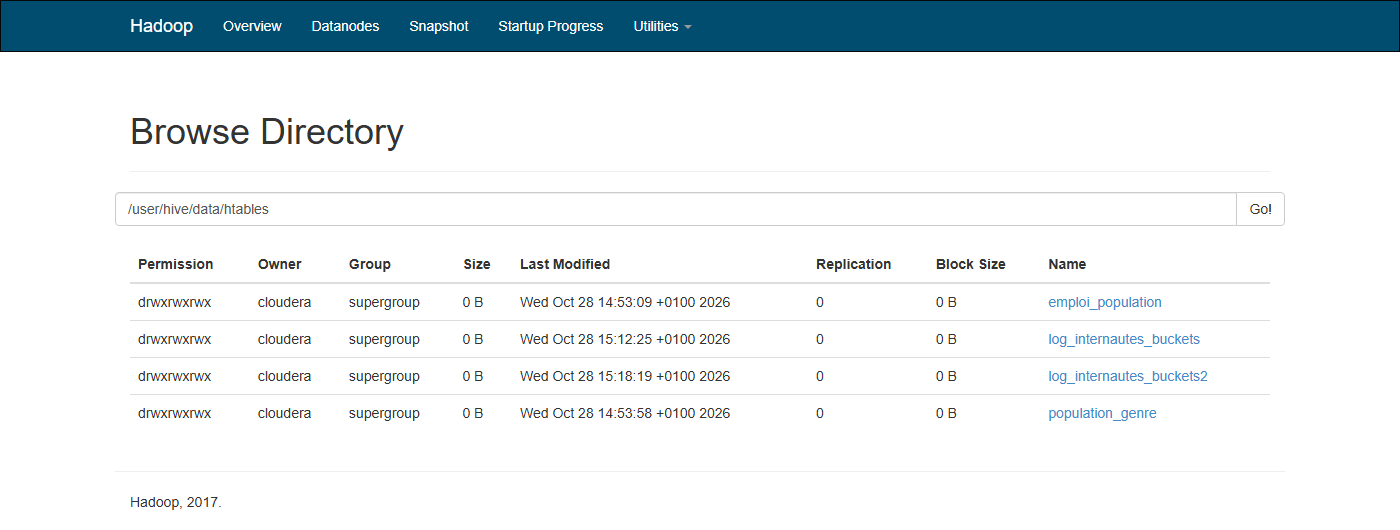
\includegraphics{contents/img/captures/hdfs_htables.png}}\par\nobreak\smallskip
\small\textit{Figure~2 -- Navigateur HDFS~: dossier \texttt{/user/hive/data/htables} après la création de la base.}
\end{center}

\subsection*{2. Table externe et suppression}
\phantomsection
\addcontentsline{toc}{subsection}{2. Table externe et suppression}

\noindent La table externe \texttt{log\_emploi\_population} décrit le fichier \texttt{emploi\_population.txt}, sans le déplacer~:

\begin{minted}{sql}
CREATE EXTERNAL TABLE IF NOT EXISTS log_emploi_population (
  genre STRING, date_naissance DATE, fonction STRING,
  salaire STRING, code_postal STRING, id INT)
COMMENT 'table intermediaire'
ROW FORMAT DELIMITED FIELDS TERMINATED BY '\073'
STORED AS TEXTFILE
LOCATION '/user/hive/data/emploi_population';
\end{minted}

\noindent \texttt{DESCRIBE FORMATTED} indique \texttt{Table Type: EXTERNAL\_TABLE} et \texttt{field.delim = ;}. Le \texttt{SELECT *} renvoie bien les 12~lignes (extrait réel)~:

\begin{tableau}{|>{\raggedright\arraybackslash}p{\dimexpr0.14\linewidth-2\tabcolsep-1.2\arrayrulewidth\relax}|>{\raggedright\arraybackslash}p{\dimexpr0.20\linewidth-2\tabcolsep-1.2\arrayrulewidth\relax}|>{\raggedright\arraybackslash}p{\dimexpr0.20\linewidth-2\tabcolsep-1.2\arrayrulewidth\relax}|>{\raggedright\arraybackslash}p{\dimexpr0.20\linewidth-2\tabcolsep-1.2\arrayrulewidth\relax}|>{\raggedleft\arraybackslash}p{\dimexpr0.14\linewidth-2\tabcolsep-1.2\arrayrulewidth\relax}|>{\raggedleft\arraybackslash}p{\dimexpr0.12\linewidth-2\tabcolsep-1.2\arrayrulewidth\relax}|}
\rowcolor{tabentete}\normalfont \textbf{genre} & \normalfont \textbf{date\_naissance} & \normalfont \textbf{fonction} & \normalfont \textbf{salaire} & \normalfont \textbf{code\_postal} & \normalfont \textbf{id} \\ \hline
Feminin & 1989-03-03 & Aide-soignant & 20000euro/an & 59000 & 1 \\ \hline
Masculin & 1982-02-15 & Informaticien & 35000euro/an & 80000 & 2 \\ \hline
Feminin & 1968-04-26 & Infermiere & 22000euro/an & 77000 & 3 \\ \hline
\multicolumn{6}{|c|}{\dots} \\ \hline
Feminin & 1996-03-20 & Musicienne & 41000euro/an & 6000 & 12 \\ \hline
\end{tableau}

\noindent \textbf{Que devient le fichier si on supprime la table~?} Le script exécute \texttt{DROP TABLE log\_emploi\_population}, puis \texttt{dfs -ls /user/hive/data/emploi\_population}. Le fichier \texttt{emploi\_population.txt} (634 octets) est toujours là~: Hive n'a supprimé que la description. La table recréée retrouve ses données immédiatement.

\subsection*{3. Table finale par CTAS}
\phantomsection
\addcontentsline{toc}{subsection}{3. Table finale par CTAS}

\noindent La table \texttt{emploi\_population} est créée à partir de la table intermédiaire avec un \textit{CREATE TABLE AS SELECT}~: le genre est réduit à son initiale (F ou M) et la date de naissance devient un âge.

\begin{minted}{sql}
CREATE TABLE IF NOT EXISTS emploi_population AS
SELECT SUBSTR(genre, 1, 1) AS sexe,
       ROUND(DATEDIFF(CURRENT_TIMESTAMP(), date_naissance) / 365.2425) AS age,
       fonction, salaire, code_postal, id AS Id_empl
FROM log_emploi_population;
\end{minted}

\noindent La requête garde le \texttt{CURRENT\_TIMESTAMP()} de l'énoncé, qui fonctionne dans le Hive~1.1 de Cloudera. Le \texttt{DESCRIBE} réel donne les colonnes \texttt{sexe string}, \texttt{age double}, \texttt{fonction}, \texttt{salaire}, \texttt{code\_postal} (\texttt{string}) et \texttt{id\_empl int}. L'âge est un \texttt{double} parce que \texttt{ROUND} renvoie un \texttt{double}. Extrait de la table, pour les femmes (sortie réelle de \texttt{SELECT * ... WHERE sexe = 'F'}, âges au 28~octobre 2026)~:

\begin{tableau}{|>{\centering\arraybackslash}p{\dimexpr0.10\linewidth-2\tabcolsep-1.2\arrayrulewidth\relax}|>{\raggedleft\arraybackslash}p{\dimexpr0.10\linewidth-2\tabcolsep-1.2\arrayrulewidth\relax}|>{\raggedright\arraybackslash}p{\dimexpr0.25\linewidth-2\tabcolsep-1.2\arrayrulewidth\relax}|>{\raggedright\arraybackslash}p{\dimexpr0.25\linewidth-2\tabcolsep-1.2\arrayrulewidth\relax}|>{\raggedleft\arraybackslash}p{\dimexpr0.15\linewidth-2\tabcolsep-1.2\arrayrulewidth\relax}|>{\raggedleft\arraybackslash}p{\dimexpr0.15\linewidth-2\tabcolsep-1.2\arrayrulewidth\relax}|}
\rowcolor{tabentete}\normalfont \textbf{sexe} & \normalfont \textbf{age} & \normalfont \textbf{fonction} & \normalfont \textbf{salaire} & \normalfont \textbf{code\_postal} & \normalfont \textbf{id\_empl} \\ \hline
F & 38,0 & Aide-soignant & 20000euro/an & 59000 & 1 \\ \hline
F & 59,0 & Infermiere & 22000euro/an & 77000 & 3 \\ \hline
F & 70,0 & Professeur & 30000euro/an & 95000 & 4 \\ \hline
F & 71,0 & Pericultrice & 38000euro/an & 76000 & 8 \\ \hline
F & 54,0 & Informaticienne & 45000euro/an & 91000 & 9 \\ \hline
F & 31,0 & Musicienne & 41000euro/an & 6000 & 12 \\ \hline
\end{tableau}

\noindent Le flux complet de la partie~1, du fichier à la table finale~:

\begin{center}
\begin{adjustbox}{max width=\linewidth}
\begin{tikzpicture}[node distance=1.0cm, every node/.style={font=\scriptsize}]
	\node[cmp=3.3cm] (f) {Fichier\\ \texttt{emploi\_population.txt}};
	\node[cmp=3.4cm, right=of f] (l) {Table externe\\ \texttt{log\_emploi\_population}\\ genre, date\_naissance, id};
	\node[cmp=3.3cm, right=of l, fill=title2!12, draw=title1] (e) {Table \texttt{emploi\_population}\\ sexe, age, id\_empl};
	\draw[flux] (f) -- node[above]{\texttt{LOCATION}} (l);
	\draw[flux] (l) -- node[above]{CTAS} (e);
	\node[below=0.9cm of l, text width=3.2cm, align=left, draw=gray!50, fill=gray!6, rounded corners=2pt, inner sep=3pt] (t) {\texttt{genre} $\rightarrow$ \texttt{sexe}\\ (\texttt{SUBSTR}, 1 lettre)\\ \texttt{date\_naissance} $\rightarrow$ \texttt{age}\\ (\texttt{DATEDIFF} / 365,2425)\\ \texttt{id} $\rightarrow$ \texttt{id\_empl}};
	\draw[flux, dashed] (t) -- (l.south);
	\draw[flux, dashed] (t) -| (e.south);
\end{tikzpicture}
\end{adjustbox}\par\nobreak\smallskip
\small\textit{Figure~3 -- Passage de la table intermédiaire à la table finale~: colonnes transformées par le CTAS.}
\end{center}

\subsection*{4. Table interne et suppression}
\phantomsection
\addcontentsline{toc}{subsection}{4. Table interne et suppression}

\noindent La table interne \texttt{personne} reçoit le fichier \texttt{personne.txt}, copié au préalable dans l'entrepôt Hive. L'énoncé laisse sa définition à compléter~: nous retenons deux colonnes, \texttt{id INT} et \texttt{nom STRING} (le fichier a une troisième colonne, les prénoms, ignorée par la table).

\begin{minted}{sql}
CREATE TABLE IF NOT EXISTS personne (id INT, nom STRING)
COMMENT 'Table interne personne'
ROW FORMAT DELIMITED FIELDS TERMINATED BY '\073' STORED AS TEXTFILE;
LOAD DATA INPATH '/user/hive/warehouse/personne.txt' OVERWRITE INTO TABLE personne;
DROP TABLE personne;
dfs -ls /user/hive/data/htables;
\end{minted}

\noindent \texttt{LOAD DATA INPATH} \textbf{déplace} le fichier~: il quitte \texttt{/user/hive/warehouse} pour \texttt{/user/hive/data/htables/personne}. Après le \texttt{DROP TABLE}, le \texttt{dfs -ls} de \texttt{/user/hive/data/htables} ne montre plus que le dossier \texttt{emploi\_population}~: contrairement à la table externe, la table interne emporte ses données.

\begin{tableau}{|>{\bfseries\raggedright\arraybackslash}p{\dimexpr0.24\linewidth-2\tabcolsep-1.2\arrayrulewidth\relax}|>{\raggedright\arraybackslash}p{\dimexpr0.38\linewidth-2\tabcolsep-1.2\arrayrulewidth\relax}|>{\raggedright\arraybackslash}p{\dimexpr0.38\linewidth-2\tabcolsep-1.2\arrayrulewidth\relax}|}
\rowcolor{tabentete} & \normalfont \textbf{Table externe} & \normalfont \textbf{Table interne} \\ \hline
Propriétaire des fichiers & Les fichiers existent avant la table & Hive (entrepôt ou emplacement de la base) \\ \hline
\texttt{DROP TABLE} & Supprime la description, garde les fichiers & Supprime la description et les fichiers \\ \hline
\texttt{LOAD DATA INPATH} & Non utilisé (\texttt{LOCATION}) & Déplace le fichier vers la table \\ \hline
Exemple du workshop & \texttt{log\_emploi\_population} & \texttt{personne} \\ \hline
\end{tableau}

\begin{center}
\begin{adjustbox}{max width=\linewidth}
\begin{tikzpicture}[node distance=0.5cm, every node/.style={font=\scriptsize},
	titre/.style={font=\small\bfseries},
	zone/.style={draw=title1, rounded corners=2pt, fill=title2!8, text width=5.6cm, align=left, inner sep=4pt},
	fic/.style={draw=gray, rounded corners=2pt, fill=white, font=\scriptsize\ttfamily, inner sep=3pt},
	rouge/.style={draw=red!60!black, rounded corners=2pt, fill=red!8, text width=5.6cm, align=left, inner sep=4pt}]
	\node[titre] (te) at (0,0) {Table externe};
	\node[titre] (ti) at (7,0) {Table interne};
	\node[zone, below=0.3cm of te] (ze) {Description dans le metastore\\ \texttt{LOCATION '/user/hive/data/emploi\_population'}};
	\node[fic, below=0.5cm of ze] (fe) {emploi\_population.txt};
	\node[zone, below=0.3cm of ti] (zi) {Description dans le metastore\\ (emplacement de la base ou entrepôt)};
	\node[fic, below=0.5cm of zi] (fi) {personne.txt};
	\node[rouge, below=0.5cm of fe] (de) {\texttt{DROP TABLE}~: la description disparaît, \textbf{le fichier reste}.};
	\node[rouge, below=0.5cm of fi] (di) {\texttt{DROP TABLE}~: la description \textbf{et le fichier} disparaissent.};
	\draw[flux] (ze) -- node[right]{lit} (fe);
	\draw[flux] (zi) -- node[right]{possède} (fi);
	\draw[flux, dashed] (fe) -- (de);
	\draw[flux, dashed] (fi) -- (di);
	\node[font=\scriptsize\itshape, text width=5.6cm, align=left, below=0.1cm of de] {Le fichier existe avant la table~; pas de \texttt{LOAD DATA}.};
	\node[font=\scriptsize\itshape, text width=5.6cm, align=left, below=0.1cm of di] {\texttt{LOAD DATA INPATH} déplace le fichier vers le dossier de la table.};
\end{tikzpicture}
\end{adjustbox}\par\nobreak\smallskip
\small\textit{Figure~4 -- Table externe et table interne~: où sont les données et effet de \texttt{DROP TABLE}.}
\end{center}

% =====================================================================
\section*{Partie 2~: partitions et buckets}
\phantomsection
\addcontentsline{toc}{section}{Partie 2~: partitions et buckets}

\subsection*{1. Partition par sexe}
\phantomsection
\addcontentsline{toc}{subsection}{1. Partition par sexe}

\noindent Une \textbf{partition} range les lignes dans un sous-dossier par valeur d'une colonne. Une requête qui filtre sur cette colonne ne lit que le sous-dossier concerné. La table \texttt{population\_genre} est partitionnée par \texttt{sexe}~; la colonne n'est plus dans les fichiers, elle est dans le nom du dossier.

\begin{minted}{sql}
CREATE EXTERNAL TABLE population_genre (
  age INT, fonction STRING, salaire STRING, code_postal STRING, id INT)
PARTITIONED BY (sexe STRING)
ROW FORMAT DELIMITED FIELDS TERMINATED BY ',';

SET hive.exec.dynamic.partition=true;
SET hive.exec.dynamic.partition.mode=nonstrict;
INSERT OVERWRITE TABLE population_genre PARTITION (sexe)
SELECT age, fonction, salaire, code_postal, id_empl, sexe FROM emploi_population;
\end{minted}

\noindent Le mode dynamique crée les partitions à partir des valeurs lues~; le mode \texttt{nonstrict} est nécessaire parce que toutes les colonnes de partition sont dynamiques. Résultats réels~:

\begin{itemize}
	\item \texttt{SELECT DISTINCT(sexe)} renvoie \texttt{F} et \texttt{M}~;
	\item \texttt{SHOW PARTITIONS population\_genre} renvoie \texttt{sexe=F} et \texttt{sexe=M}~;
	\item le journal de l'insertion donne 6~lignes dans chaque partition (\texttt{numRows=6}, \texttt{totalSize} de 220 et 216 octets)~;
	\item \texttt{dfs -ls -R} montre un fichier \texttt{000000\_0} dans chacun des deux sous-dossiers.
\end{itemize}

\begin{center}
\begin{adjustbox}{max width=\linewidth}
\begin{tikzpicture}[
	dossier/.style={draw=title1, rounded corners=2pt, fill=title2!10, font=\scriptsize\ttfamily, inner sep=4pt},
	fichier/.style={draw=gray, rounded corners=2pt, fill=white, font=\scriptsize\ttfamily, inner sep=3pt},
	vide/.style={draw=gray!60, dashed, rounded corners=2pt, fill=gray!10, font=\scriptsize\ttfamily, inner sep=3pt, text=gray!70!black},
	lien/.style={draw=black!55, line width=0.6pt}]
	\node[dossier] (r) {/user/hive/data/htables/population\_genre};
	\node[dossier, below left=0.9cm and 0.2cm of r] (f) {sexe=F};
	\node[dossier, below right=0.9cm and 0.2cm of r] (m) {sexe=M};
	\node[fichier, below=0.7cm of f] (ff) {000000\_0 (220 o, 6 lignes)};
	\node[fichier, below=0.7cm of m] (mf) {000000\_0 (216 o, 6 lignes)};
	\draw[lien] (r) -- (f); \draw[lien] (r) -- (m);
	\draw[lien] (f) -- (ff); \draw[lien] (m) -- (mf);
\end{tikzpicture}
\end{adjustbox}
\end{center}

\noindent Les deux requêtes suivantes donnent les mêmes six femmes, mais la seconde ne lit que le dossier \texttt{sexe=F}~:

\begin{minted}{sql}
SELECT * FROM emploi_population WHERE sexe = 'F';
SELECT * FROM population_genre  WHERE sexe = 'F';
\end{minted}

\begin{tableau}{|>{\ttfamily\raggedright\arraybackslash}p{\dimexpr0.30\linewidth-2\tabcolsep-1.2\arrayrulewidth\relax}|>{\raggedleft\arraybackslash}p{\dimexpr0.12\linewidth-2\tabcolsep-1.2\arrayrulewidth\relax}|>{\raggedright\arraybackslash}p{\dimexpr0.58\linewidth-2\tabcolsep-1.2\arrayrulewidth\relax}|}
\rowcolor{tabentete}\normalfont \textbf{Table} & \normalfont \textbf{Temps} & \normalfont \textbf{Mode d'exécution lu dans le journal} \\ \hline
emploi\_population (complète) & 13,949 s & Travail MapReduce, 1 mapper, aucun reducer \\ \hline
population\_genre (partition F) & 0,21 s & Aucun travail MapReduce~: lecture directe du dossier \\ \hline
\end{tableau}

\noindent Les deux temps sont lus dans la sortie réelle du rejeu final. Ils ne se comparent pas directement~: la requête sur la table complète a lancé un travail MapReduce (environ 14~s, dont l'essentiel est le démarrage du travail), alors que celle sur la partition a été lue sans MapReduce, par un simple parcours du dossier (0,21~s). Sur douze lignes, le gain vient de la \textit{méthode} et non du volume~: la partition évite de lancer un travail et de lire les fichiers de l'autre sexe. Ce gain grandit avec le volume des données.

\subsection*{2. Partitions et buckets sur les internautes}
\phantomsection
\addcontentsline{toc}{subsection}{2. Partitions et buckets sur les internautes}

\noindent Un \textbf{bucket} répartit les lignes d'une table (ou d'une partition) dans un nombre fixe de fichiers, selon le hachage d'une colonne~: bucket = (hachage \& \texttt{Integer.MAX\_VALUE}) modulo 4. Pour un entier, le hachage est sa valeur~; pour une chaîne, c'est \texttt{String.hashCode()}. Les buckets servent à répartir la charge, à échantillonner (\texttt{TABLESAMPLE}) et à accélérer les jointures.

\noindent La table intermédiaire \texttt{log\_internautes} (17~lignes) est lue depuis le dossier \texttt{/user/hive/data/internautes}. Une première table réunit les deux techniques~: une partition par date, et dans chaque partition 4~buckets sur \texttt{id\_internaute}.

\begin{minted}{sql}
SET hive.enforce.bucketing=true;
CREATE TABLE log_internautes_buckets (
  id_internaute INT, prenom STRING, site_consulte STRING, pays STRING)
PARTITIONED BY (date_consultation STRING)
CLUSTERED BY (id_internaute) INTO 4 BUCKETS
ROW FORMAT DELIMITED FIELDS TERMINATED BY '\073' STORED AS TEXTFILE;

INSERT OVERWRITE TABLE log_internautes_buckets PARTITION (date_consultation)
SELECT id_internaute, prenom, site_consulte, pays, date_consultation FROM log_internautes;
\end{minted}

\noindent \texttt{DESCRIBE FORMATTED} confirme \texttt{Num Buckets: 4} et \texttt{Bucket Columns: [id\_internaute]}~; \texttt{SHOW PARTITIONS} liste les trois dates. Le travail MapReduce utilise 4~reducers, un par bucket. L'arborescence réelle relevée par \texttt{dfs -ls -R} est la suivante (taille de chaque fichier en octets)~:

\begin{center}
\begin{adjustbox}{max width=\linewidth}
\begin{tikzpicture}[
	dossier/.style={draw=title1, rounded corners=2pt, fill=title2!10, font=\scriptsize\ttfamily, inner sep=4pt},
	fichier/.style={draw=gray, rounded corners=2pt, fill=white, font=\scriptsize\ttfamily, inner sep=3pt, minimum width=2.6cm},
	vide/.style={draw=gray!60, dashed, rounded corners=2pt, fill=gray!10, font=\scriptsize\ttfamily, inner sep=3pt, text=gray!70!black, minimum width=2.6cm},
	lien/.style={draw=black!55, line width=0.6pt}]
	\node[dossier] (r) at (0,0) {/user/hive/data/htables/log\_internautes\_buckets};
	\node[dossier] (p1) at (-5.6,-1.8) {date\_consultation=27-04-2016};
	\node[dossier] (p2) at (0,-1.8) {date\_consultation=28-04-2016};
	\node[dossier] (p3) at (5.6,-1.8) {date\_consultation=29-04-2016};
	\foreach \p in {p1,p2,p3} \draw[lien] (r) -- (\p);
	% 27-04
	\node[fichier] (a0) at (-5.6,-3.2) {000000\_0 (24 o)};
	\node[fichier] (a1) at (-5.6,-4.0) {000001\_0 (93 o)};
	\node[vide] (a2) at (-5.6,-4.8) {000002\_0 (0 o)};
	\node[vide] (a3) at (-5.6,-5.6) {000003\_0 (0 o)};
	% 28-04
	\node[fichier] (b0) at (0,-3.2) {000000\_0 (54 o)};
	\node[vide] (b1) at (0,-4.0) {000001\_0 (0 o)};
	\node[fichier] (b2) at (0,-4.8) {000002\_0 (94 o)};
	\node[fichier] (b3) at (0,-5.6) {000003\_0 (54 o)};
	% 29-04
	\node[fichier] (c0) at (5.6,-3.2) {000000\_0 (23 o)};
	\node[fichier] (c1) at (5.6,-4.0) {000001\_0 (22 o)};
	\node[vide] (c2) at (5.6,-4.8) {000002\_0 (0 o)};
	\node[fichier] (c3) at (5.6,-5.6) {000003\_0 (49 o)};
	\foreach \p/\q in {p1/a0,p2/b0,p3/c0} \draw[lien] (\p) -- (\q);
\end{tikzpicture}
\end{adjustbox}
\end{center}

\noindent Les fichiers en pointillés sont des buckets vides (0~octet)~: ils existent quand même, parce que Hive crée toujours autant de fichiers que de buckets. Le bucket de chaque ligne se calcule avec la règle ci-dessus~; les tailles lues correspondent au calcul (la répartition par bucket est calculée avec cette règle, le total de chaque partition est lu dans \texttt{numRows})~:

\begin{tableau}{|>{\raggedright\arraybackslash}p{\dimexpr0.22\linewidth-2\tabcolsep-1.2\arrayrulewidth\relax}|>{\raggedleft\arraybackslash}p{\dimexpr0.15\linewidth-2\tabcolsep-1.2\arrayrulewidth\relax}|>{\raggedleft\arraybackslash}p{\dimexpr0.15\linewidth-2\tabcolsep-1.2\arrayrulewidth\relax}|>{\raggedleft\arraybackslash}p{\dimexpr0.15\linewidth-2\tabcolsep-1.2\arrayrulewidth\relax}|>{\raggedleft\arraybackslash}p{\dimexpr0.15\linewidth-2\tabcolsep-1.2\arrayrulewidth\relax}|>{\raggedleft\arraybackslash}p{\dimexpr0.18\linewidth-2\tabcolsep-1.2\arrayrulewidth\relax}|}
\rowcolor{tabentete}\normalfont \textbf{Partition} & \normalfont \textbf{Bucket 0} & \normalfont \textbf{Bucket 1} & \normalfont \textbf{Bucket 2} & \normalfont \textbf{Bucket 3} & \normalfont \textbf{Total (lu)} \\ \hline
27-04-2016 & 1 & 4 & 0 & 0 & 5 \\ \hline
28-04-2016 & 2 & 0 & 4 & 2 & 8 \\ \hline
29-04-2016 & 1 & 1 & 0 & 2 & 4 \\ \hline
\end{tableau}

\noindent Pour le 27 avril, les buckets 2 et 3 sont vides~: avec cinq lignes et quatre buckets, un bucket sans ligne est normal. Cela confirme la remarque de l'énoncé. Les deux autres dates ont aussi un bucket vide.

\noindent Les captures du navigateur HDFS confirment ces fichiers~: les trois dossiers de partition (Figure~5), puis le contenu de la partition du 27~avril, où \texttt{000002\_0} et \texttt{000003\_0} (les buckets 2 et 3) font bien 0~octet (Figure~6).

\begin{center}
\begin{minipage}{\linewidth}\centering
\adjustbox{max width=\linewidth, max height=0.28\textheight}{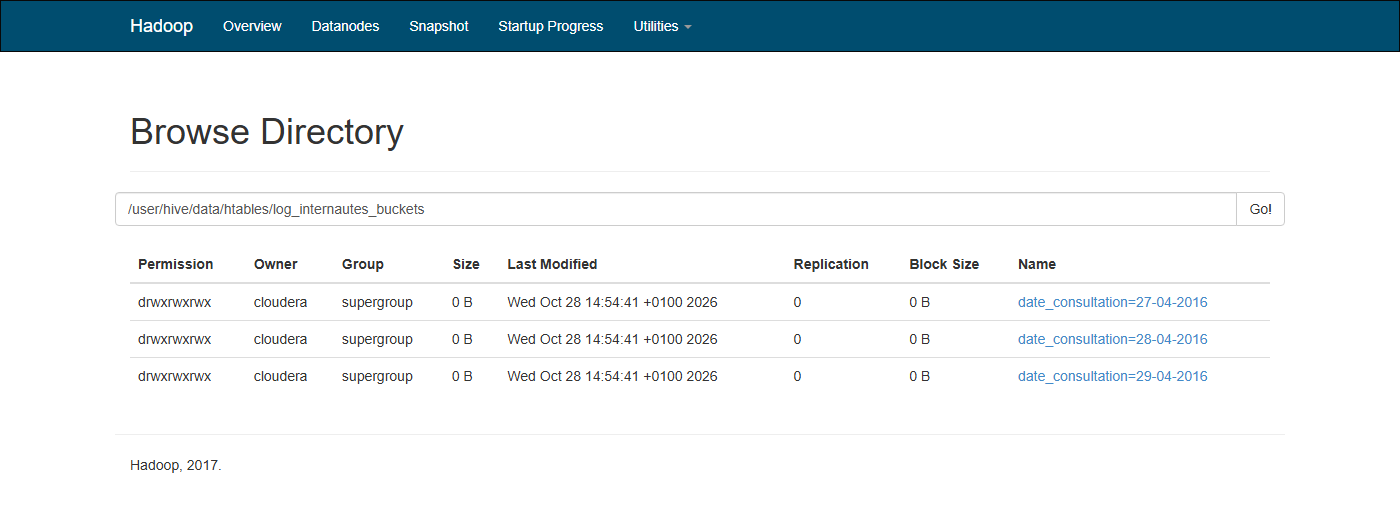
\includegraphics{contents/img/captures/hdfs_buckets.png}}\par\nobreak\smallskip
\small\textit{Figure~5 -- Navigateur HDFS~: les trois partitions de \texttt{log\_internautes\_buckets}.}\par\medskip
\adjustbox{max width=\linewidth, max height=0.28\textheight}{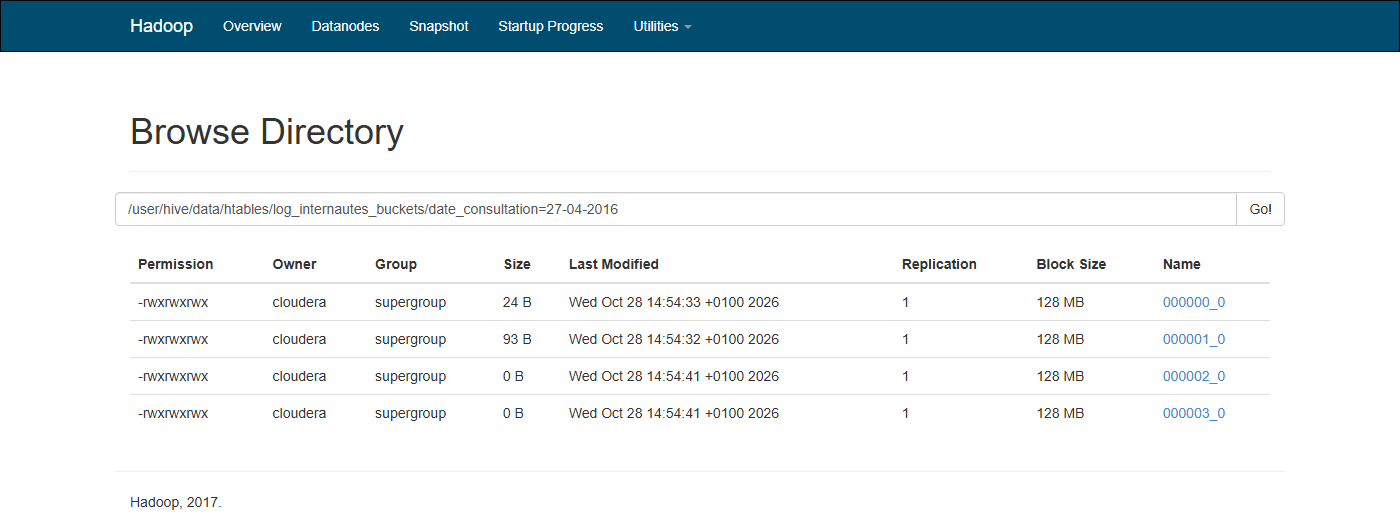
\includegraphics{contents/img/captures/hdfs_buckets_partition.png}}\par\nobreak\smallskip
\small\textit{Figure~6 -- Partition du 27-04-2016~: \texttt{000000\_0} (24~o), \texttt{000001\_0} (93~o), \texttt{000002\_0} et \texttt{000003\_0} (0~o).}
\end{minipage}
\end{center}

\subsection*{3. Buckets sur le pays, sans partition}
\phantomsection
\addcontentsline{toc}{subsection}{3. Buckets sur le pays, sans partition}

\noindent La seconde table répartit toutes les lignes en 4~buckets selon \texttt{pays}, sans partition~:

\begin{minted}{sql}
CREATE TABLE log_internautes_buckets2 (
  id_internaute INT, prenom STRING, site_consulte STRING,
  date_consultation STRING, pays STRING)
CLUSTERED BY (pays) INTO 4 BUCKETS
ROW FORMAT DELIMITED FIELDS TERMINATED BY '\073' STORED AS TEXTFILE;
\end{minted}

\noindent Le journal donne \texttt{numFiles=4, numRows=17, totalSize=600}. Les fichiers lus par \texttt{dfs -ls -R}~:

\begin{tableau}{|>{\ttfamily\raggedright\arraybackslash}p{\dimexpr0.20\linewidth-2\tabcolsep-1.2\arrayrulewidth\relax}|>{\raggedleft\arraybackslash}p{\dimexpr0.15\linewidth-2\tabcolsep-1.2\arrayrulewidth\relax}|>{\raggedright\arraybackslash}p{\dimexpr0.65\linewidth-2\tabcolsep-1.2\arrayrulewidth\relax}|}
\rowcolor{tabentete}\normalfont \textbf{Fichier} & \normalfont \textbf{Taille (o)} & \normalfont \textbf{Pays qu'il contient} \\ \hline
000000\_0 & 84 & AUSTRALIA (2 lignes, vérifié par \texttt{TABLESAMPLE}) \\ \hline
000001\_0 & 0 & Aucun \\ \hline
000002\_0 & 305 & JAPAN, UK, US (9 lignes, calculé par le hachage)
\\ \hline
000003\_0 & 211 & CHINA, INDIA (6 lignes, calculé par le hachage)
\\ \hline
\end{tableau}

\noindent Six pays se partagent quatre buckets~: le hachage ne garantit pas une répartition égale. Le bucket 1 reste vide, et le bucket 2 regroupe trois pays. Le choix de la colonne de bucket compte~: avec peu de valeurs distinctes, la répartition est inégale. La requête \texttt{TABLESAMPLE(BUCKET 1 OUT OF 4 ON pays)} ne lit que le premier fichier~; elle renvoie bien les deux lignes d'Australie (Ricky et Michel).

% =====================================================================
\section*{Partie 3~: analyse des salaires}
\phantomsection
\addcontentsline{toc}{section}{Partie 3~: analyse des salaires}

\subsection*{1. Préparation}
\phantomsection
\addcontentsline{toc}{subsection}{1. Préparation}

\noindent La base \texttt{analyse\_salaires} contient trois tables externes, une par fichier. Les fichiers \texttt{fonction\_employes} et \texttt{salaire\_employes} ont une ligne d'en-tête, ignorée grâce à \texttt{skip.header.line.count}~:

\begin{minted}{sql}
CREATE EXTERNAL TABLE salaire_employes (
  sexe STRING, secteur STRING, salaire STRING, code_postal INT, id_empl INT)
ROW FORMAT DELIMITED FIELDS TERMINATED BY '\073' STORED AS TEXTFILE
LOCATION '/user/hive/data/salaire'
TBLPROPERTIES ("skip.header.line.count"="1");
\end{minted}


\begin{center}
\begin{adjustbox}{max width=\linewidth}
\begin{tikzpicture}
	\node[sous=3.8cm] (E) at (-5,0) {\tb{employes}{\pk{id\_empl} INT\\ nom STRING\\ prenom STRING\\ date\_naissance STRING}};
	\node[sous=3.8cm] (F) at (0,0) {\tb{fonction\_employes}{\pk{id\_empl} INT\\ annee\_embauche INT\\ fonction STRING}};
	\node[sous=3.8cm] (S) at (5,0) {\tb{salaire\_employes}{\pk{id\_empl} INT\\ sexe STRING\\ secteur STRING\\ salaire STRING\\ code\_postal INT}};
	\draw[lien] (E.east) -- node[above, font=\tiny]{id\_empl} (F.west);
	\draw[lien] (F.east) -- node[above, font=\tiny]{id\_empl} (S.west);
\end{tikzpicture}
\end{adjustbox}\par\nobreak\smallskip
\small\textit{Figure~7 -- Les trois tables externes de \texttt{analyse\_salaires}, reliées par la clé \texttt{id\_empl} (33 lignes chacune).}
\end{center}

\noindent Les trois \texttt{SELECT COUNT(*)} renvoient bien \textbf{33} lignes chacune (\texttt{employes}, \texttt{fonction\_employes}, \texttt{salaire\_employes}), lu sur Hive. Le salaire est une chaîne du type \texttt{20000euro/an}. Une vue utilitaire, ajoutée hors énoncé, joint les trois tables et convertit le salaire en nombre~; l'expérience est l'année courante moins l'année d'embauche.

\begin{minted}{sql}
CREATE VIEW v_employes_complet AS
SELECT e.id_empl, e.nom, e.prenom, s.sexe, s.secteur,
       CAST(REGEXP_REPLACE(s.salaire, '[^0-9]', '') AS INT) AS salaire_num,
       s.code_postal, f.annee_embauche, f.fonction,
       YEAR(CURRENT_DATE()) - f.annee_embauche AS experience
FROM employes e
JOIN fonction_employes f ON e.id_empl = f.id_empl
JOIN salaire_employes s ON e.id_empl = s.id_empl;
\end{minted}

\noindent La regex supprime tout ce qui n'est pas un chiffre~: elle traite aussi la faute \texttt{42000euo/an} de la ligne~26. Sur la machine Cloudera, les jointures échouent avec la conversion automatique en jointure locale (\texttt{MapredLocalTask}, erreur Java)~: le script ajoute \texttt{SET hive.auto.convert.join=false}. Les résultats ci-dessous sont les résultats réels de Hive, lus dans la sortie du rejeu complet du script~; chaque requête MapReduce prend de 20~s à 2~ou 3~minutes sur la machine virtuelle.

\noindent L'interface YARN (\texttt{quickstart.cloudera:8088}) liste les travaux MapReduce lancés par les requêtes~: les 62 travaux de la session ont le statut \textit{SUCCEEDED}.

\begin{center}
\adjustbox{max width=\linewidth, max height=0.35\textheight}{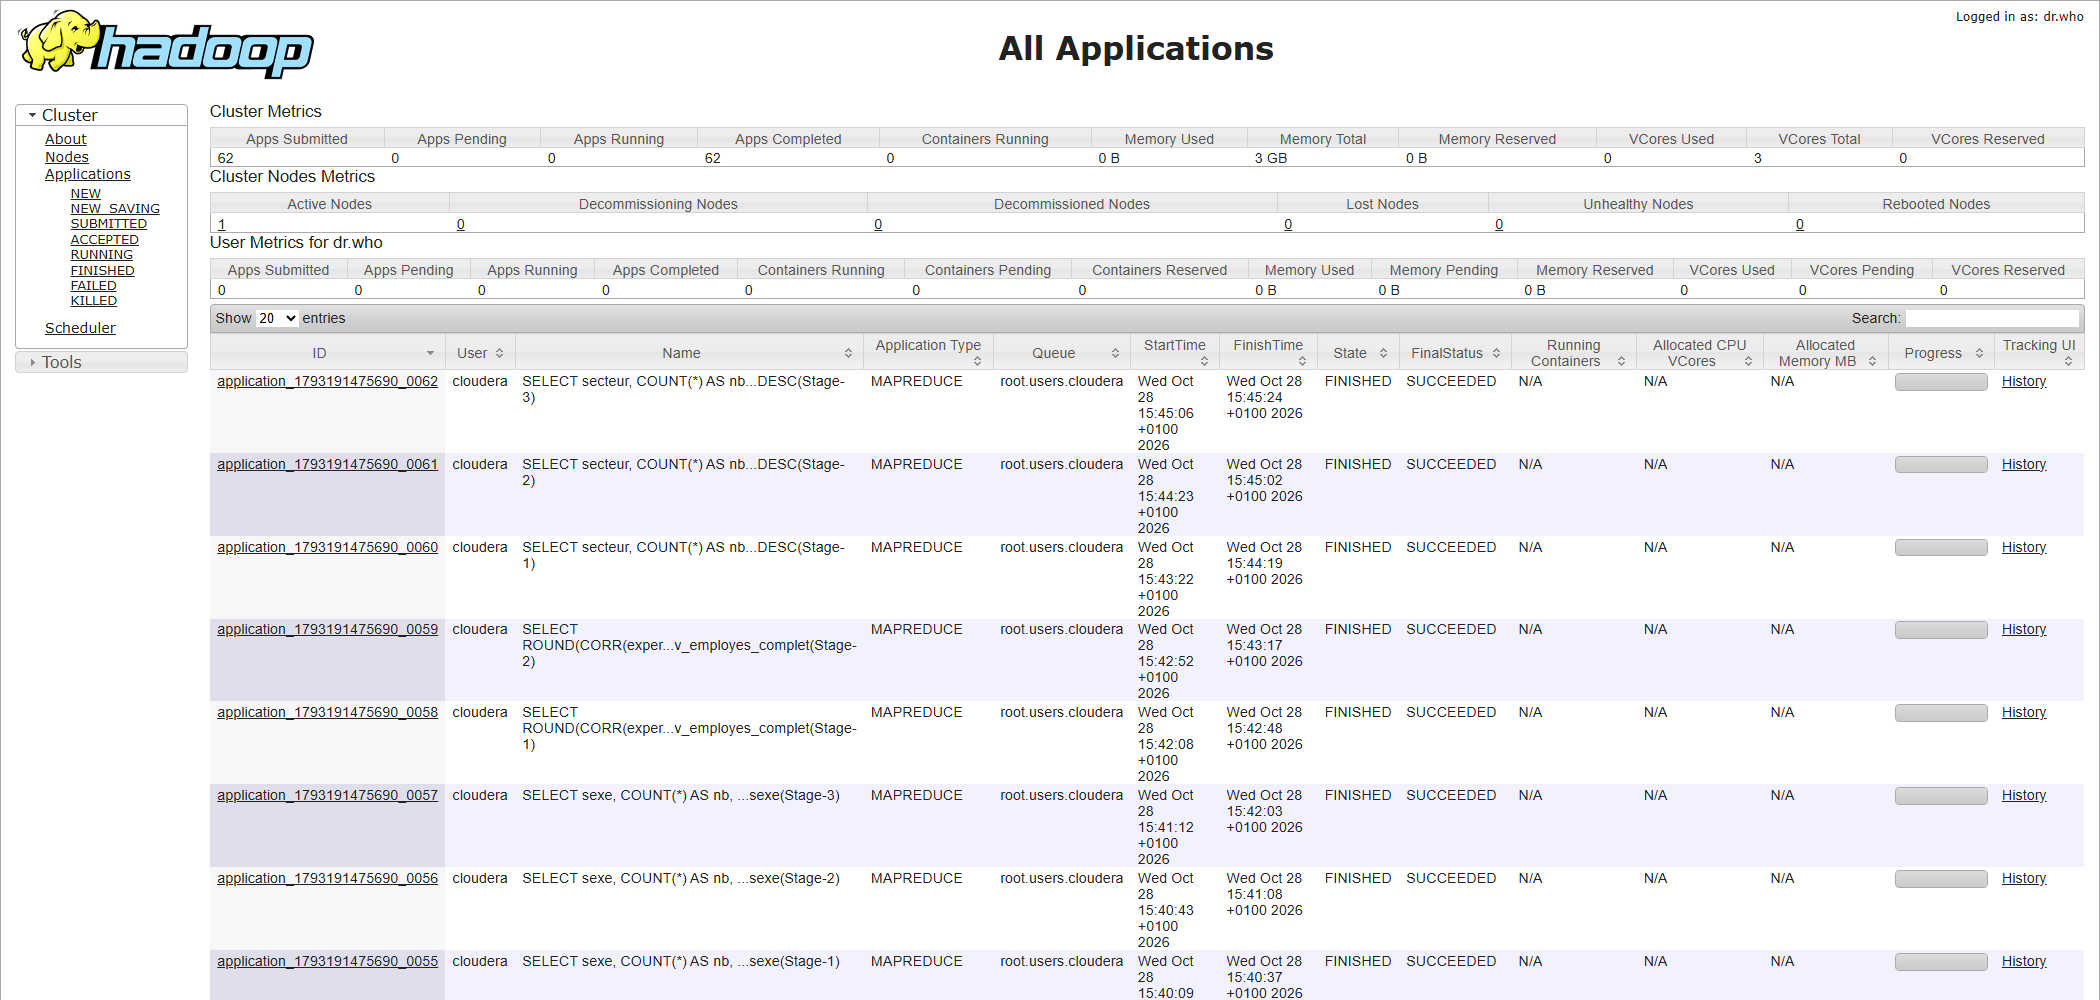
\includegraphics{contents/img/captures/yarn_jobs.png}}\par\nobreak\smallskip
\small\textit{Figure~8 -- YARN, \textit{All Applications}~: travaux MapReduce lancés par les requêtes Hive (62 travaux \textit{SUCCEEDED}).}
\end{center}

\subsection*{2. Q1 à Q7}
\phantomsection
\addcontentsline{toc}{subsection}{2. Q1 à Q7}

\noindent \textbf{Q1. Combien d'employés ont été embauchés après 2019~?}

\begin{minted}{sql}
SELECT COUNT(*) AS nb_embauches_apres_2019
FROM fonction_employes WHERE annee_embauche > 2019;
\end{minted}

\noindent Résultat lu sur Hive~: \textbf{7} employés. L'année 2019 est exclue, d'après le sens de « après ».

\medskip
\noindent \textbf{Q2. Quelles paires employé-secteur ont un salaire supérieur à 35\,000~euros par an~?}

\begin{minted}{sql}
SELECT id_empl, nom, prenom, secteur, salaire_num
FROM v_employes_complet WHERE salaire_num > 35000 ORDER BY id_empl;
\end{minted}

\noindent 24 lignes (les salaires de 35\,000 exactement, ids 2 et 27, sont exclus). Les huit premières~:

\begin{tableau}{|>{\raggedleft\arraybackslash}p{\dimexpr0.07\linewidth-2\tabcolsep-1.2\arrayrulewidth\relax}|>{\raggedright\arraybackslash}p{\dimexpr0.22\linewidth-2\tabcolsep-1.2\arrayrulewidth\relax}|>{\raggedright\arraybackslash}p{\dimexpr0.26\linewidth-2\tabcolsep-1.2\arrayrulewidth\relax}|>{\raggedright\arraybackslash}p{\dimexpr0.30\linewidth-2\tabcolsep-1.2\arrayrulewidth\relax}|>{\raggedleft\arraybackslash}p{\dimexpr0.15\linewidth-2\tabcolsep-1.2\arrayrulewidth\relax}|}
\rowcolor{tabentete}\normalfont \textbf{id} & \normalfont \textbf{nom} & \normalfont \textbf{prenom} & \normalfont \textbf{secteur} & \normalfont \textbf{salaire} \\ \hline
5 & VANDENDRIESSCHE & HENRI PIERRE & industrie & 45\,000 \\ \hline
6 & WACCUS & GUILLAUME AUGUSTIN & profession juridique privé & 70\,000 \\ \hline
7 & CHARPENTIER & PIERRE & sante & 45\,000 \\ \hline
8 & DEKYDTSPOTTER & PAULETTE OCTAVIE & soin et education & 38\,000 \\ \hline
9 & SOLEYMIEUX & FRANCINE JEANNE & industrie & 45\,000 \\ \hline
11 & TERZIS & PASCAL PIERRE & sante & 55\,000 \\ \hline
12 & HOUMADI OILI & FATIMA & arts et spectacle & 41\,000 \\ \hline
13 & LALLEMANT & ETIENNE BERNARD PIERRE & transports aeriens & 144\,000 \\ \hline
\multicolumn{5}{|c|}{\dots} \\ \hline
\end{tableau}

\noindent La plus haute valeur est 200\,000 (id~30, profession juridique privé).

\medskip
\noindent \textbf{Q3. Quels employés du secteur éducation ont été recrutés après 2010~?} L'énoncé crée une vue avec \texttt{employes} et \texttt{fonction\_employes}~; le secteur est dans \texttt{salaire\_employes}, d'où une jointure de plus.

\begin{minted}{sql}
CREATE VIEW vue_employes_apres_2010 AS
SELECT e.id_empl, e.nom, e.prenom, f.annee_embauche, f.fonction
FROM employes e JOIN fonction_employes f ON e.id_empl = f.id_empl
WHERE f.annee_embauche > 2010;

SELECT v.id_empl, v.nom, v.prenom, v.annee_embauche, v.fonction
FROM vue_employes_apres_2010 v JOIN salaire_employes s ON v.id_empl = s.id_empl
WHERE s.secteur = 'education' ORDER BY v.id_empl;
\end{minted}

\begin{center}
\begin{adjustbox}{max width=\linewidth}
\begin{tikzpicture}[node distance=1cm, every node/.style={font=\scriptsize}]
	\node[cmp=2.6cm] (e) {\texttt{employes}};
	\node[cmp=2.6cm, below=0.5cm of e] (f) {\texttt{fonction\_employes}\\ filtre \texttt{annee\_embauche > 2010}};
	\node[cmp=4.6cm, right=1.4cm of e, yshift=-0.9cm, fill=title2!12, draw=title1] (v) {Vue \texttt{vue\_employes\_apres\_2010}\\ id\_empl, nom, prenom, annee\_embauche, fonction};
	\node[cmp=2.6cm, below=0.5cm of f] (s) {\texttt{salaire\_employes}\\ filtre \texttt{secteur = 'education'}};
	\node[cmp=2.6cm, right=1.4cm of v, fill=orange!25] (r) {Résultat Q3\\ 1 employé};
	\draw[flux] (e) -- (v.west |- e.east); \draw[flux] (f) -- (v);
	\draw[flux] (v) -- node[above]{jointure} (r);
	\draw[flux] (s.east) -| node[pos=0.25, below]{\texttt{id\_empl}} (r.south);
\end{tikzpicture}
\end{adjustbox}\par\nobreak\smallskip
\small\textit{Figure~9 -- Question Q3~: la vue de l'énoncé (employés recrutés après 2010) est jointe à \texttt{salaire\_employes} pour filtrer le secteur.}
\end{center}

\noindent Une seule personne~: \textbf{CANSALADE Charlotte Henriette} (id~19, embauchée en 2018, fonction « ressource humaine »).
Le filtre est une égalité stricte~: le secteur « soin et education » n'est pas retenu.

\medskip
\noindent \textbf{Q4. Quel employé a le plus d'expérience~?} L'expérience est l'année courante moins l'année d'embauche. La requête garde les ex-aequo avec \texttt{RANK()}~; Hive~1.1 n'accepte pas de sous-requête scalaire.

\begin{minted}{sql}
SELECT id_empl, nom, prenom, annee_embauche, fonction, experience
FROM (SELECT id_empl, nom, prenom, annee_embauche, fonction, experience,
             RANK() OVER (ORDER BY experience DESC) AS rang
      FROM v_employes_complet) t
WHERE rang = 1;
\end{minted}

\noindent \textbf{TODORIS Vassiliki} (id~4, professeur, embauchée en 1970), soit 56~ans d'expérience en 2026, sans ex-aequo.

\medskip
\noindent \textbf{Q5. Quel est le salaire moyen des employés~?}

\begin{minted}{sql}
SELECT ROUND(AVG(salaire_num), 2) AS salaire_moyen FROM v_employes_complet;
\end{minted}

\noindent \textbf{55\,696,97~euros par an} (1\,838\,000 pour 33 employés).

\medskip
\noindent \textbf{Q6. Quelles sont les fonctions des femmes, par année d'embauche~?} \texttt{COLLECT\_SET} regroupe les fonctions distinctes de chaque année dans une liste.

\begin{minted}{sql}
SELECT annee_embauche, COLLECT_SET(fonction) AS fonctions
FROM v_employes_complet WHERE sexe = 'F'
GROUP BY annee_embauche ORDER BY annee_embauche;
\end{minted}

\begin{tableau}{|>{\raggedleft\arraybackslash}p{\dimexpr0.10\linewidth-2\tabcolsep-1.2\arrayrulewidth\relax}|>{\raggedright\arraybackslash}p{\dimexpr0.40\linewidth-2\tabcolsep-1.2\arrayrulewidth\relax}|>{\raggedleft\arraybackslash}p{\dimexpr0.10\linewidth-2\tabcolsep-1.2\arrayrulewidth\relax}|>{\raggedright\arraybackslash}p{\dimexpr0.40\linewidth-2\tabcolsep-1.2\arrayrulewidth\relax}|}
\rowcolor{tabentete}\normalfont \textbf{Année} & \normalfont \textbf{Fonctions} & \normalfont \textbf{Année} & \normalfont \textbf{Fonctions} \\ \hline
1970 & professeur & 2011 & chercheur en chimie \\ \hline
1977 & pericultrice & 2015 & aide-soignant \\ \hline
1984 & transporteur & 2018 & musicienne, ressource humaine \\ \hline
1987 & infermiere, secretaire, professeur & 2020 & infermiere, comptable \\ \hline
1990 & pediatre & 2021 & phamacienne \\ \hline
2010 & informaticienne & 2022 & technicien \\ \hline
\end{tableau}

\noindent Les listes sont données dans l'ordre renvoyé par Hive~; cet ordre n'est pas garanti.

\medskip
\noindent \textbf{Q7. Quelles paires <prénom, fonction> concernent les employés qui habitent Paris~?} Le code postal doit commencer par 75.

\begin{minted}{sql}
SELECT prenom, fonction, code_postal
FROM v_employes_complet WHERE code_postal BETWEEN 75000 AND 75999
ORDER BY code_postal;
\end{minted}

\begin{tableau}{|>{\raggedright\arraybackslash}p{\dimexpr0.50\linewidth-2\tabcolsep-1.2\arrayrulewidth\relax}|>{\raggedright\arraybackslash}p{\dimexpr0.25\linewidth-2\tabcolsep-1.2\arrayrulewidth\relax}|>{\raggedleft\arraybackslash}p{\dimexpr0.25\linewidth-2\tabcolsep-1.2\arrayrulewidth\relax}|}
\rowcolor{tabentete}\normalfont \textbf{prenom} & \normalfont \textbf{fonction} & \normalfont \textbf{code\_postal} \\ \hline
DOUGLAS LOUIS LEON & taxi & 75000 \\ \hline
PIERRE & veterinaire & 75780 \\ \hline
\end{tableau}

\noindent La colonne \texttt{code\_postal} est ajoutée au \texttt{SELECT}~: Hive~1.1 refuse un \texttt{ORDER BY} sur une colonne absente du \texttt{SELECT}. Le code 75780 n'est pas un code postal parisien, mais il passe le filtre 75xxx. Le prénom contient tous les prénoms de l'état civil.

\subsection*{3. Q8 à Q10 et conclusion}
\phantomsection
\addcontentsline{toc}{subsection}{3. Q8 à Q10 et conclusion}

\noindent \textbf{Q8. Y a-t-il une différence de salaire entre les femmes et les hommes~?} Le salaire seul ne tient pas compte de l'ancienneté. Le ratio retenu est la somme des salaires divisée par la somme des années d'expérience, par sexe.

\begin{minted}{sql}
SELECT sexe, COUNT(*) AS nb, SUM(salaire_num) AS somme_salaires,
       SUM(experience) AS somme_experience,
       ROUND(SUM(salaire_num) / SUM(experience), 2) AS ratio_salaire_par_annee_exp,
       ROUND(AVG(salaire_num), 2) AS salaire_moyen
FROM v_employes_complet GROUP BY sexe ORDER BY sexe;
\end{minted}

\begin{tableau}{|>{\centering\arraybackslash}p{\dimexpr0.10\linewidth-2\tabcolsep-1.2\arrayrulewidth\relax}|>{\raggedleft\arraybackslash}p{\dimexpr0.10\linewidth-2\tabcolsep-1.2\arrayrulewidth\relax}|>{\raggedleft\arraybackslash}p{\dimexpr0.22\linewidth-2\tabcolsep-1.2\arrayrulewidth\relax}|>{\raggedleft\arraybackslash}p{\dimexpr0.20\linewidth-2\tabcolsep-1.2\arrayrulewidth\relax}|>{\raggedleft\arraybackslash}p{\dimexpr0.18\linewidth-2\tabcolsep-1.2\arrayrulewidth\relax}|>{\raggedleft\arraybackslash}p{\dimexpr0.20\linewidth-2\tabcolsep-1.2\arrayrulewidth\relax}|}
\rowcolor{tabentete}\normalfont \textbf{sexe} & \normalfont \textbf{nb} & \normalfont \textbf{Somme salaires} & \normalfont \textbf{Somme exp.} & \normalfont \textbf{Ratio} & \normalfont \textbf{Salaire moyen} \\ \hline
F & 16 & 644\,000 & 379 & 1\,699,21 & 40\,250,00 \\ \hline
M & 17 & 1\,194\,000 & 332 & 3\,596,39 & 70\,235,29 \\ \hline
\end{tableau}


\begin{center}
\begin{minipage}{0.48\textwidth}
\centering
\begin{tikzpicture}
\begin{axis}[ybar, width=\linewidth, height=5.2cm, symbolic x coords={F,M}, xtick=data, ymin=0, enlarge x limits=0.5, bar width=0.8cm,
	ylabel={Salaire moyen (euros par an)}, xlabel={Sexe}, ylabel style={font=\scriptsize}, tick label style={font=\scriptsize}, scaled y ticks=false, yticklabel style={/pgf/number format/fixed, /pgf/number format/1000 sep=\,},
	nodes near coords, nodes near coords style={font=\tiny}, every node near coord/.append style={/pgf/number format/fixed, /pgf/number format/1000 sep=\,}]
\addplot[fill=title1!70] coordinates {(F,40250) (M,70235)};
\end{axis}
\end{tikzpicture}
\end{minipage}\hfill
\begin{minipage}{0.48\textwidth}
\centering
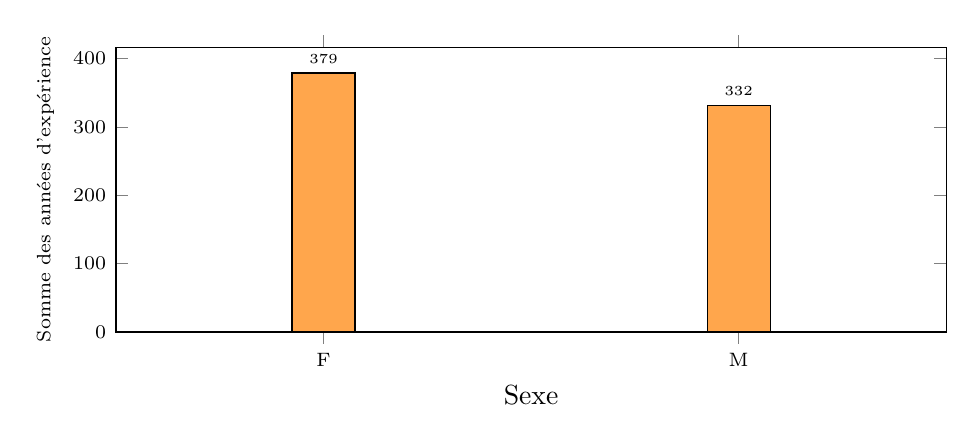
\begin{tikzpicture}
\begin{axis}[ybar, width=\linewidth, height=5.2cm, symbolic x coords={F,M}, xtick=data, ymin=0, enlarge x limits=0.5, bar width=0.8cm,
	ylabel={Somme des années d'expérience}, xlabel={Sexe}, ylabel style={font=\scriptsize}, tick label style={font=\scriptsize},
	nodes near coords, nodes near coords style={font=\tiny}]
\addplot[fill=orange!70] coordinates {(F,379) (M,332)};
\end{axis}
\end{tikzpicture}
\end{minipage}\par\nobreak\smallskip
\small\textit{Figure~10 -- Q8~: salaire moyen et somme des années d'expérience, par sexe (16 femmes, 17 hommes).}
\end{center}

\noindent Le salaire moyen des hommes est supérieur de près de 30\,000~euros à celui des femmes. Le ratio des hommes est 2,12 fois celui des femmes, alors que les femmes cumulent plus d'années d'expérience (379 contre 332). L'écart n'est donc pas expliqué par l'ancienneté~: il se creuse quand on la prend en compte. L'échantillon est de 33 personnes et sans test statistique~: c'est un constat, pas une preuve.

\medskip
\needspace{8\baselineskip}
\noindent \textbf{Q9. L'expérience influence-t-elle le salaire~?} La fonction \texttt{CORR} donne le coefficient de corrélation de Pearson.

\begin{minted}{sql}
SELECT ROUND(CORR(experience, salaire_num), 4) AS correlation_experience_salaire
FROM v_employes_complet;
\end{minted}

\noindent Résultat~: \textbf{0,0886}.
La corrélation est positive mais très faible (proche de~0)~: sur ces données, l'expérience n'explique presque pas le salaire.

\begin{center}
\begin{adjustbox}{max width=\linewidth}
\begin{tikzpicture}
\begin{axis}[width=12cm, height=7cm, xlabel={Expérience (années)}, ylabel={Salaire (euros par an)}, xmin=0, xmax=60, ymin=0, ymax=220000, grid=major, grid style={gray!25},
	scaled y ticks=false, yticklabel style={/pgf/number format/fixed, /pgf/number format/1000 sep=\,}, tick label style={font=\scriptsize}, label style={font=\small}]
\addplot[only marks, mark=*, mark size=1.8pt, color=title1] coordinates {
(11,20000) (20,35000) (39,22000) (56,30000) (5,45000) (9,70000) (16,45000) (49,38000) (16,45000) (28,30000) (6,55000) (8,41000) (7,144000) (6,41000) (5,75000) (4,25000) (6,37000) (5,80000) (8,28000) (8,65000) (16,25000) (36,80000) (26,57000) (20,38000) (42,40000) (15,42000) (39,35000) (39,45000) (48,90000) (46,200000) (16,120000) (30,55000) (26,40000)
};
\end{axis}
\end{tikzpicture}
\end{adjustbox}\par\nobreak\smallskip
\small\textit{Figure~11 -- Q9~: salaire en fonction de l'expérience pour les 33 employés (corrélation de Pearson~: 0,0886). Le nuage est dispersé, sans tendance nette.}
\end{center}

\medskip
\needspace{8\baselineskip}
\noindent \textbf{Q10. Le secteur influence-t-il le salaire~?}

\begin{minted}{sql}
SELECT secteur, COUNT(*) AS nb, ROUND(AVG(salaire_num), 2) AS salaire_moyen,
       ROUND(AVG(experience), 2) AS experience_moyenne
FROM v_employes_complet GROUP BY secteur ORDER BY salaire_moyen DESC;
\end{minted}

\begin{tableau}{|>{\raggedright\arraybackslash}p{\dimexpr0.55\linewidth-2\tabcolsep-1.2\arrayrulewidth\relax}|>{\raggedleft\arraybackslash}p{\dimexpr0.10\linewidth-2\tabcolsep-1.2\arrayrulewidth\relax}|>{\raggedleft\arraybackslash}p{\dimexpr0.18\linewidth-2\tabcolsep-1.2\arrayrulewidth\relax}|>{\raggedleft\arraybackslash}p{\dimexpr0.17\linewidth-2\tabcolsep-1.2\arrayrulewidth\relax}|}
\rowcolor{tabentete}\normalfont \textbf{Secteur} & \normalfont \textbf{nb} & \normalfont \textbf{Salaire moyen} & \normalfont \textbf{Exp. moyenne} \\ \hline
profession juridique privé & 2 & 135\,000,00 & 27,50 \\ \hline
transports aeriens & 2 & 132\,000,00 & 11,50 \\ \hline
transport & 2 & 85\,000,00 & 26,50 \\ \hline
fabrication et distribution des patisserie-viennoiserie & 1 & 65\,000,00 & 8,00 \\ \hline
pharmaceutique & 2 & 58\,500,00 & 10,00 \\ \hline
agriculture & 2 & 43\,500,00 & 27,00 \\ \hline
sante & 7 & 42\,571,43 & 19,14 \\ \hline
education & 4 & 39\,500,00 & 33,25 \\ \hline
industrie & 4 & 35\,000,00 & 10,25 \\ \hline
\multicolumn{4}{|c|}{\dots (16 secteurs au total)} \\ \hline
\end{tableau}


\begin{center}
\begin{adjustbox}{max width=\linewidth}
\begin{tikzpicture}
\begin{axis}[xbar, width=11cm, height=9.5cm, xmin=0, xmax=150000, bar width=5pt,
	xlabel={Salaire moyen (euros par an)}, ylabel={Secteur},
	symbolic y coords={profession juridique prive, transports aeriens, transport, patisserie-viennoiserie, pharmaceutique, agriculture, sante, arts et spectacle, transport et entroposage, budgetisation, education, soin et education, commerce, expert comptable, industrie, fonction publique},
	ytick=data, y dir=reverse, tick label style={font=\tiny}, label style={font=\small}, scaled x ticks=false, xticklabel style={/pgf/number format/fixed, /pgf/number format/1000 sep=\,}, xmajorgrids, grid style={gray!25},
	nodes near coords, nodes near coords style={font=\tiny}, every node near coord/.append style={/pgf/number format/fixed, /pgf/number format/1000 sep=\,}]
\addplot[fill=title1!70] coordinates {
(135000,profession juridique prive) (132000,transports aeriens) (85000,transport) (65000,patisserie-viennoiserie) (58500,pharmaceutique) (43500,agriculture) (42571,sante) (41000,arts et spectacle) (40000,transport et entroposage) (40000,budgetisation) (39500,education) (38000,soin et education) (38000,commerce) (37000,expert comptable) (35000,industrie) (35000,fonction publique)
};
\end{axis}
\end{tikzpicture}
\end{adjustbox}\par\nobreak\smallskip
\small\textit{Figure~12 -- Q10~: salaire moyen par secteur, du plus élevé (en haut) au plus bas (16 secteurs).}
\end{center}

\noindent La capture Hue montre la requête et ses 16~lignes de résultat (56,30~s). La valeur \texttt{19.140000000000001} de l'expérience moyenne du secteur « sante » est un artefact d'affichage du type \texttt{double}~: il s'agit bien de 19,14.

\begin{center}
\adjustbox{max width=\linewidth, max height=0.35\textheight}{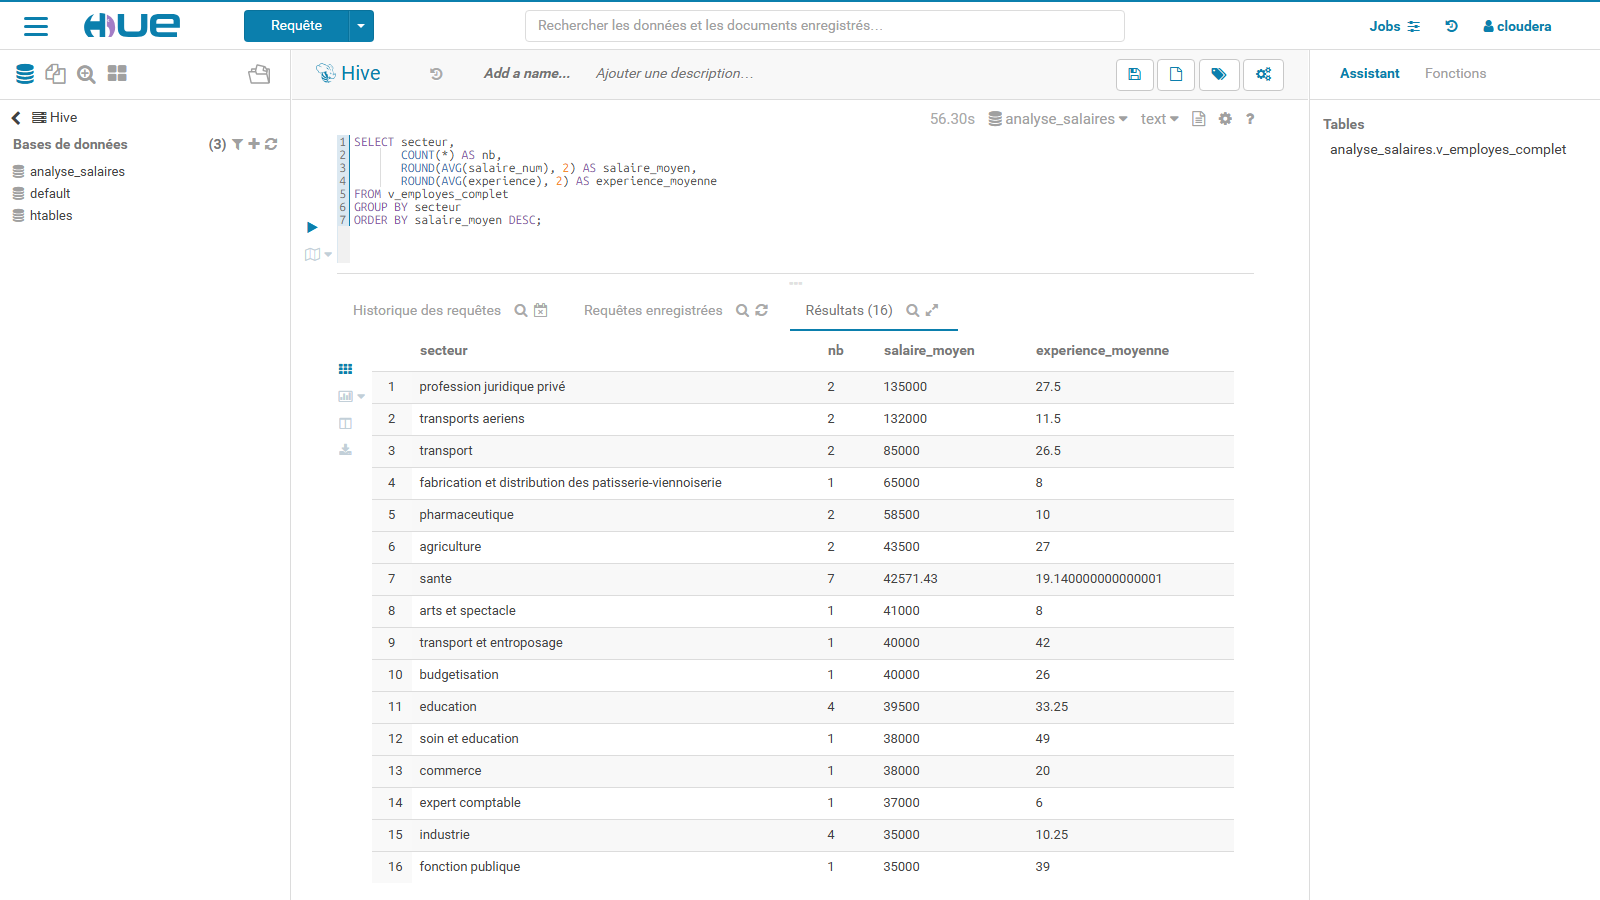
\includegraphics{contents/img/captures/hue_q10.png}}\par\nobreak\smallskip
\small\textit{Figure~13 -- Hue, éditeur Hive~: requête Q10 et résultat (16 secteurs).}
\end{center}

\noindent Les moyennes vont de 35\,000 à 135\,000~euros. Les secteurs les mieux payés (juridique, transports aériens, transport) n'ont pas les employés les plus expérimentés~: le transport aérien a 11,5 ans d'expérience en moyenne. \textbf{Conclusion Q8 à Q10}~: le secteur influence nettement le salaire, alors que l'expérience seule n'a pas d'effet net (Q9). Le sexe est lié à un écart important (Q8), mais il peut aussi venir du secteur~: ces données ne permettent pas de séparer les deux effets. Réserve~: neuf secteurs sur seize n'ont qu'un ou deux employés, et les valeurs de Q4, Q8, Q9 et Q10 dépendent de l'année d'exécution.

% =====================================================================
\section*{Pièges des données et écarts à l'énoncé}
\phantomsection
\addcontentsline{toc}{section}{Pièges des données et écarts à l'énoncé}

\subsection*{1. Pièges des données}
\phantomsection
\addcontentsline{toc}{subsection}{1. Pièges des données}

\noindent Les cinq premiers pièges sont décrits dans la section « Étude des données »~; le tableau donne le traitement de chacun, puis ceux qui concernent l'énoncé et les requêtes.

\begin{tableau}{|>{\bfseries\raggedright\arraybackslash}p{\dimexpr0.22\linewidth-2\tabcolsep-1.2\arrayrulewidth\relax}|>{\raggedright\arraybackslash}p{\dimexpr0.78\linewidth-2\tabcolsep-1.2\arrayrulewidth\relax}|}
\rowcolor{tabentete}\normalfont \textbf{Piège} & \normalfont \textbf{Traitement appliqué} \\ \hline
Encodage & Conversion en UTF-8 (copies dans \texttt{data/}) \\ \hline
Fins de ligne & Conversion en LF (\texttt{dos2unix}) avant la copie sur la VM \\ \hline
En-têtes & \texttt{skip.header.line.count=1} sur \texttt{fonction\_employes} et \texttt{salaire\_employes} \\ \hline
Dates & Colonnes en \texttt{DATE} pour AAAA-MM-JJ~; \texttt{employes.txt} en \texttt{STRING}, inutilisé dans les requêtes \\ \hline
Salaire en texte & \texttt{CAST(REGEXP\_REPLACE(salaire, '[\textasciicircum 0-9]', '') AS INT)}, qui corrige aussi \texttt{euo/an} \\ \hline
Noms de fichiers & L'énoncé cite des fichiers \texttt{.csv} (\texttt{employes1.csv}...)~; les fichiers sont des \texttt{.txt}, noms réels utilisés \\ \hline
Colonnes en trop & \texttt{personne.txt} a trois colonnes, l'énoncé n'en demande que deux~: le troisième champ est ignoré \\ \hline
Prénoms & La colonne \texttt{prenom} de \texttt{employes} contient tous les prénoms de l'état civil~: à signaler (Q7) \\ \hline
Code 75780 & Passe le filtre 75xxx de Q7 sans être parisien~: conservé, signalé \\ \hline
\end{tableau}

\subsection*{2. Écarts à l'énoncé}
\phantomsection
\addcontentsline{toc}{subsection}{2. Écarts à l'énoncé}

\begin{itemize}[midpenalty=0, endpenalty=0]
	\item \textbf{\texttt{CURRENT\_TIMESTAMP()}}~: la fonction existe dans le Hive~1.1 de Cloudera~; la syntaxe de l'énoncé est conservée dans le CTAS. Les questions utilisent \texttt{YEAR(CURRENT\_DATE())} pour l'année courante.
	\item \textbf{Emplacement de la table externe}~: \texttt{/user/hive/data/emploi\_population} au lieu de \texttt{/user/hive/data}. Ce dernier dossier contient des sous-dossiers que Hive ne sait pas lire sur une table texte (erreur \textit{Not a file}).
	\item \textbf{Nom de table}~: l'énoncé demande de supprimer \texttt{log\_salaire\_population}, qui n'existe pas~; la table s'appelle \texttt{log\_emploi\_population}.
	\item \textbf{Base \texttt{htables}}~: l'énoncé la crée deux fois (\texttt{CREATE DATABASE}, puis \texttt{CREATE DATABASE IF NOT EXISTS ... LOCATION}, sans effet sur une base existante). Le script ne garde que la seconde, précédée d'un \texttt{DROP DATABASE IF EXISTS ... CASCADE} pour pouvoir être rejoué.
	\item \textbf{Rejeu de la partie~1}~: \texttt{LOAD DATA} déplace \texttt{personne.txt} hors de l'entrepôt~; il faut relancer \texttt{00\_hdfs.sh} avant de rejouer le script.
	\item \textbf{Table \texttt{personne}}~: définition laissée libre par l'énoncé, choisie à deux colonnes (\texttt{id}, \texttt{nom}).
	\item \textbf{\texttt{population\_genre}}~: table externe sans \texttt{LOCATION}, comme dans l'énoncé~; ses partitions sont écrites dans le dossier de la base \texttt{htables}. La colonne \texttt{age INT} reçoit un \texttt{double}~: conversion implicite.
	\item \textbf{Q3}~: la vue de l'énoncé ne contient pas le secteur, d'où une jointure avec \texttt{salaire\_employes}.
	\item \textbf{Q4}~: \texttt{RANK()} plutôt qu'une sous-requête scalaire, non acceptée par Hive~1.1.
	\item \textbf{Séparateur \texttt{';'}}~: le client Hive coupe l'instruction au point-virgule placé dans la chaîne (erreur \textit{ParseException ... expecting StringLiteral near 'BY'}). Le script écrit \texttt{'\textbackslash 073'}, le code octal du point-virgule.
	\item \textbf{Jointures}~: \texttt{SET hive.auto.convert.join=false} en tête du script 03, parce que la conversion en jointure locale échoue sur la machine (\texttt{MapredLocalTask}, \textit{NullPointerException}).
	\item \textbf{Q7}~: \texttt{ORDER BY id\_empl} échoue (\textit{Invalid table alias or column reference}) car la colonne n'est pas dans le \texttt{SELECT}~; la requête sélectionne \texttt{code\_postal} et trie dessus.
	\item \textbf{Ajouts}~: la vue \texttt{v\_employes\_complet}, des commandes \texttt{dfs -ls} dans les scripts pour voir les fichiers sans l'interface web, et \texttt{SET hive.enforce.bucketing=true} (valable en Hive~1.1, supprimé en Hive~4).
	\item \textbf{Dépendance à la date}~: Q4, Q8, Q9, Q10 et l'âge de \texttt{emploi\_population} changent avec la date d'exécution (ici, l'année 2026 et le 28~octobre 2026).
\end{itemize}

% =====================================================================
\section*{Conclusion}
\phantomsection
\addcontentsline{toc}{section}{Conclusion}

\noindent Ce workshop a présenté trois outils de Hive pour manipuler des données dans HDFS~:
\begin{enumerate}
	\item \textbf{les tables externes et internes}~: la table externe décrit des fichiers qui lui survivent, la table interne possède les siens et les supprime avec elle~;
	\item \textbf{les partitions et les buckets}~: la partition range les lignes par valeur d'une colonne, ce qui évite de lire les autres dossiers~; le bucket répartit les lignes en un nombre fixe de fichiers par hachage, avec des fichiers vides et des répartitions inégales quand il y a peu de lignes ou de valeurs distinctes~;
	\item \textbf{l'analyse en HiveQL}~: jointures, agrégats, fonctions de fenêtrage (\texttt{RANK}), listes (\texttt{COLLECT\_SET}) et corrélation (\texttt{CORR}) sur trois tables d'employés.
\end{enumerate}

\noindent L'analyse montre que le secteur pèse nettement sur le salaire, et que l'expérience seule n'a presque pas d'effet. Un écart entre les femmes et les hommes apparaît, sans que l'on puisse le séparer de l'effet du secteur sur 33 personnes. Hive~1.1 impose ses limites (fonctions absentes, sous-requêtes, jointures locales)~: plusieurs requêtes de l'énoncé ont dû être adaptées, et chaque écart est noté. Enfin, les données ont demandé un nettoyage avant toute requête (encodage, fins de ligne, en-têtes), comme dans le workshop précédent.
